\subsection{Carte du jeu}

\subsubsection{Première soutenance}

    La carte étant un élément crucial du jeu, au même titre que les mécaniques, 
    il nous a semblé important de faire des schémas et que le groupe soit d'accord sur la direction artistique,
    afin que Paul, la personne en charge de la map, puisse être sûr de la vision de la carte du jeu avant de commencer.
    commencer. Ainsi, la carte finalement retenue devait avoir suffisamment de 
    relief pour rendre les échelles intéressantes, et suffisamment spacieuse pour 
    pouvoir la remplir avec au moins 150 personnages non-joueurs (afin de pimenter le jeu).
    Dans un premier temps, une forme ronde avait été retenue pour la carte, mais 
    a ensuite évolué pour une forme en L, cette dernière rendant l’environnement 
    plus naturel et augmentant les chances des personnages de se croiser.


    \begin{figure}[hbt!]
        \centering
        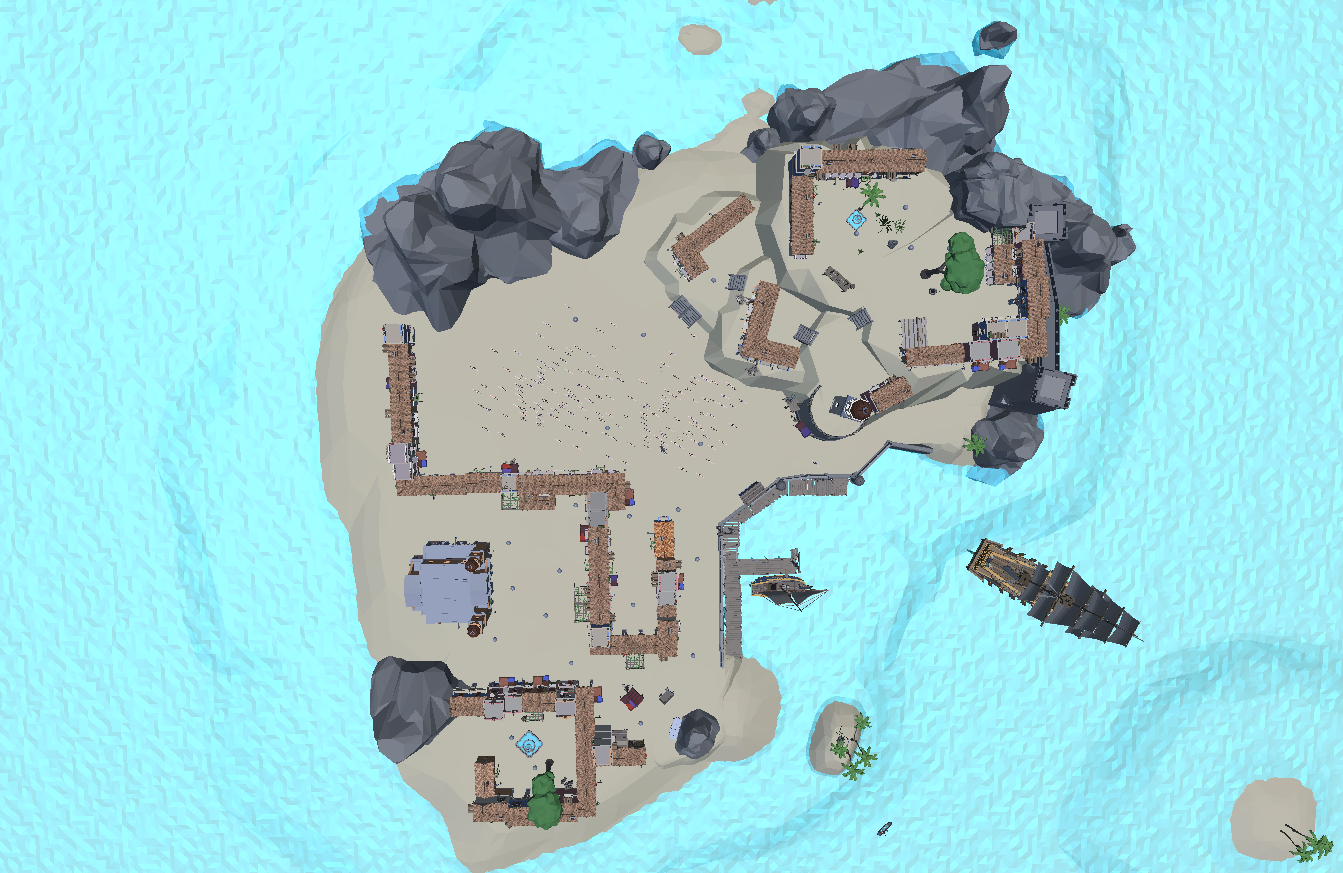
\includegraphics[scale=0.42]{fly_view.png}
        \caption{Vue aérienne de la carte}
    \end{figure}

    Ensuite, afin d’ajouter du relief à la carte, une colline a été créée. 
    Cette dernière s’étend sur environ un quart de la carte, et possède quatre 
    niveaux afin d’en permettre l’accès par de petits escaliers successifs. 
    Une colline étant un terrain irrégulier, il a été décidé que les bâtiments 
    placés sur cette dernière ne seraient pas parallèles, mais répartis afin de 
    créer un imbroglio de maisons rappelant le style méditerranéen dont les îles 
    comme celle-ci sont inspirées.


    \begin{figure}[hbt!]
        \centering
        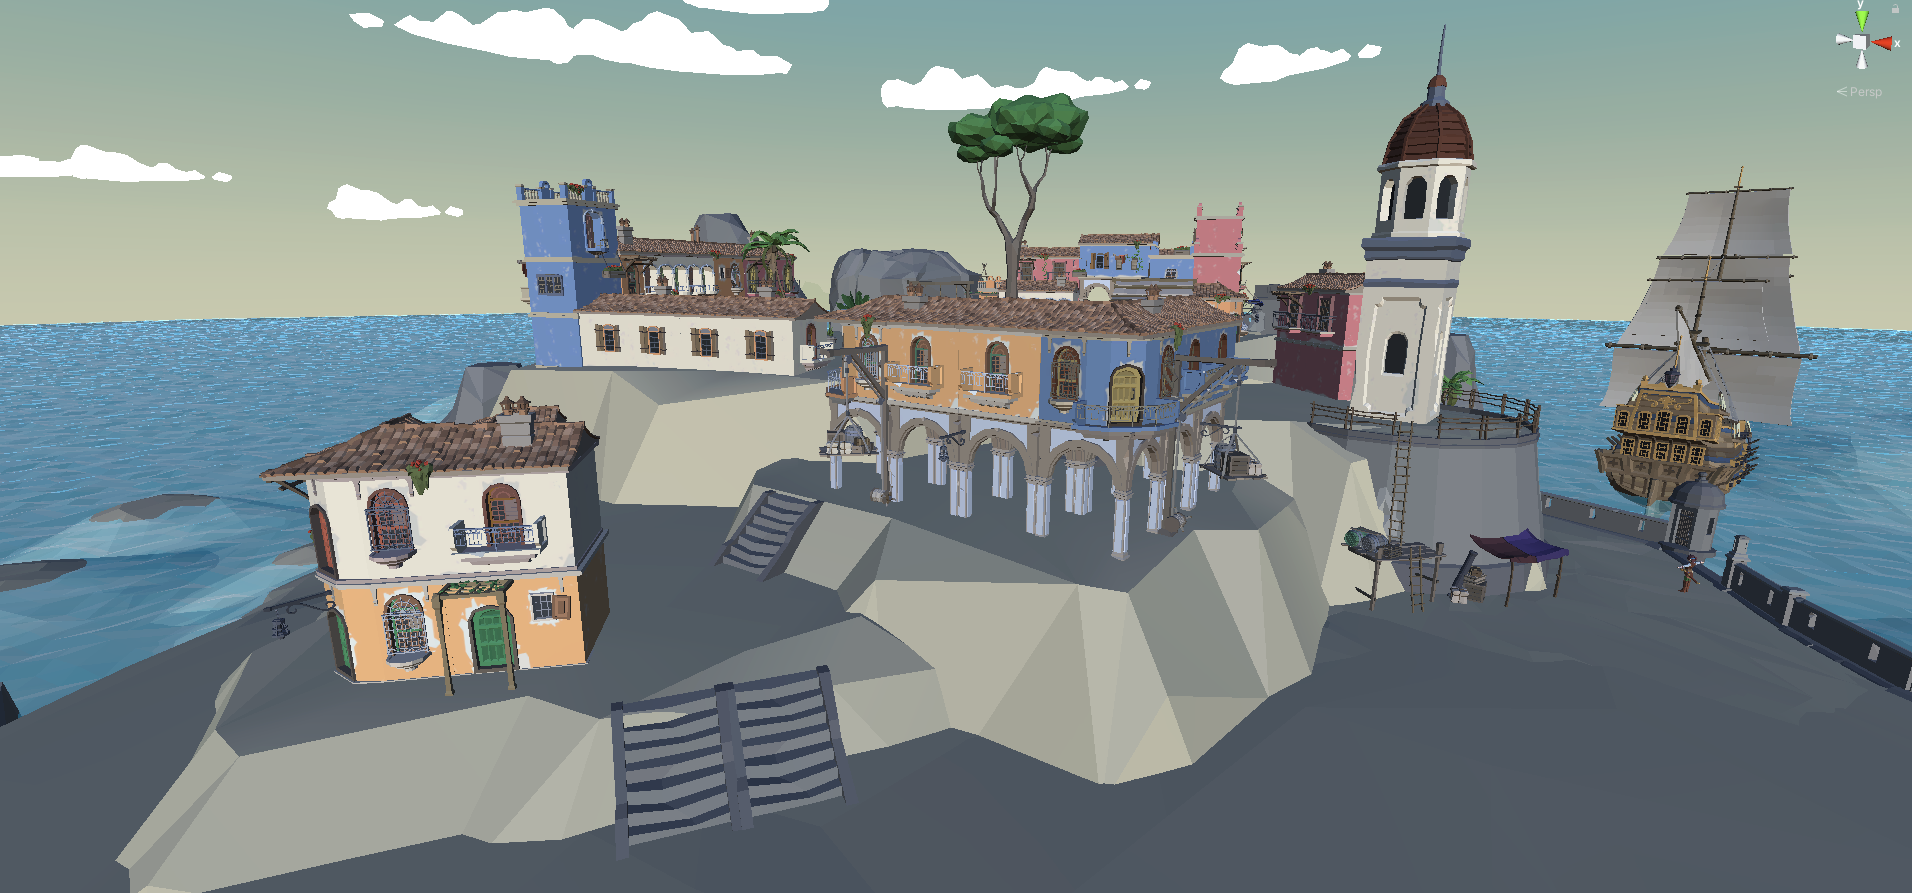
\includegraphics[scale=0.3]{hill.png}
        \caption{Colline de la carte, organisée par étages}
    \end{figure}


    Enfin, l’architecture de la ville elle-même devait aussi avoir une influence 
    ibérique, les maisons ont été dessinées basses et organisées autour de places et 
    marchés animés. Les tonnelles et les nombreuses lanternes rendent l’environnement 
    plus chaleureux, et les arcades, dotées de portes qui se ferment lorsqu’un joueur 
    les passe en courant, ajoutent une mécanique de fuite au jeu\footnote{Cf. Gameplay/Environnement}. L’organisation du 
    village se fait autour de la place de l’église, qui fait office de place du marché.\\


\subsubsection{Deuxième soutenance}

    La carte est désormais finie, et de nouveaux éléments ont été ajoutés, comme un shader animé (créé avec l'outil Shader Graph) pour l'eau,
    faite par Dov, ou encore de nouvelles lumières dynamiques. Elle est aussi dotée de nombreuses échelles, qui permettent de fuir ses poursuivants 
    de façon discrète, ainsi que de venelles reliant les avenues.
    En outre, les nombreux NPC ainsi que les marchandises exposées au milieu des rues font aussi de bonnes diversions.
    Enfin, l'ajout d'escaliers offrant un second accès à la colline permettent non seulement de désengorger la butte, envahie par les NPC, mais aussi 
    de redynamiser la digue qui était jusque là exempte de tout intérêt : pas de bâtiments, pas de cachettes...

    Mais la principale nouveauté est le mode nuit : en effet, il est désormais possible de passer du jour à la nuit grâce à de simples boutons-radios. 
    Le mode nuit applique des effets de post-processing à toutes les textures de la carte, et assombrissant les couleurs et en appliquant certains effets 
    visuels se traduisant en jeu par un environnement plus sombre (deonc nocturne). 
    Ce mode nuit permet de faire ressortir la beauté de la ville endormie, tout en ajoutant un côté angoissant aux parties,
    qui deviennent \textit{de facto} beaucoup plus animées.

    Il reste à peaufiner les détails, comme l'ajout de hautes herbes dans les rues, le placement de torches utilisant 
    la lumière dynamique (mode jour / nuit) ou encore le réajustement de petites erreurs de placements.

\subsubsection{Dernière soutenance}

    % à écrire



